\begin{table}[h]
\centering
\caption{Fitting parameters for the prompt curve. The background is $C=11.4 \pm 0.1$.}
\begin{tabular}{c| ccc}
\toprule
Peak&$A\pm 100$&$\mu$&$\sigma$\\
\midrule
  1&$ 17641$&$ 898.1\pm 0.4 $&$ 42.7\pm 0.4$\\
  2&$ 17954$&$ 1484.4\pm 0.4 $&$ 43.4\pm 0.4$\\
  3&$ 19171$&$ 2087.3\pm 0.4$&$ 44.3\pm 0.4$\\
  4&$ 19203$&$ 2683.1\pm 0.4$&$ 44.8\pm 0.4$\\
  5&$ 18926$&$ 3279.9\pm 0.4$&$ 45.4\pm 0.4$\\
  6&$ 20017$&$ 3878.1\pm 0.4$&$ 45.1\pm 0.4$\\
  7&$ 19590$&$ 4491.0\pm 0.4$&$ 44.8\pm 0.4$\\
  8&$ 20974$&$ 5089.9\pm 0.4$&$ 44.4\pm 0.4$\\
  9&$ 19890$&$ 5685.9\pm 0.4$&$ 44.4\pm 0.4$\\
  10&$ 22073$&$ 6287.7\pm 0.3$&$ 45.6\pm 0.4$\\
  11&$ 21493$&$ 6901.9\pm 0.4$&$ 44.8\pm 0.4$\\
  12&$ 13190$&$ 7483.9\pm 0.3$&$ 25.8\pm 0.3$\\
\bottomrule
\end{tabular}
\label{tab:prompt}
\end{table}

\begin{table}[h]
\centering
\caption{Fitting parameters for the annihilation radition rate.}
\begin{tabular}{c| ccccccc}
\toprule
$T/\si{\celsius} \pm 1$ & $A_0$ & $A_\mathrm{t}$ & $\tau_0$ & $\tau_\mathrm{t}$ & $t_0$ & $\sigma$ & $BG$\\
\midrule
  27& $ 144374\pm 61210$ & $ 84165\pm 57430$ & $ 44\pm 8$ & $ 99\pm 39$ & $ 929.9\pm 0.6$ & $ 30.4\pm 0.3$ & $ 20\pm 10$ \\
  55& $ 45155\pm 5927$ & $ 74952\pm 5291$ & $ 26\pm 4$ & $ 84\pm 6$ & $ 927.8\pm 0.7$ & $ 32.2\pm 0.3$ & $ 6\pm 2$ \\
  61& $ 31577\pm 4998$ & $ 86564\pm 4290$ & $ 20\pm 5$ & $ 75\pm 4$ & $ 926\pm 1$ & $ 31.7\pm 0.4$ & $ 7\pm 2$ \\
  68& $ 49181\pm 15300$ & $ 69806\pm 14400$ & $ 34\pm 6$ & $ 86\pm 11$ & $ 923.6\pm 0.7$ & $ 31.3\pm 0.3$ & $ 7\pm 3$ \\
  78& $ 35792\pm 4993$ & $ 81462\pm 4325$ & $ 22\pm 5$ & $ 80\pm 5$ & $ 927\pm 1$ & $ 32.2\pm 0.4$ & $ 6\pm 2$ \\
  81& $ 67881\pm 19180$ & $ 52323\pm 18240$ & $ 44\pm 6$ & $ 100\pm 19$ & $ 921.1\pm 0.4$ & $ 31.1\pm 0.2$ & $ 5\pm 2$ \\
  95& $ 49622\pm 20540$ & $ 67690\pm 19690$ & $ 39\pm 8$ & $ 88\pm 13$ & $ 921.5\pm 0.5$ & $ 30.2\pm 0.3$ & $ 7\pm 2$ \\
  108& $ 36028\pm 7202$ & $ 81457\pm 6573$ & $ 28\pm 5$ & $ 83\pm 5$ & $ 924.6\pm 0.7$ & $ 31.2\pm 0.3$ & $ 7\pm 2$ \\
  121& $ 28767\pm 6071$ & $ 90120\pm 5249$ & $ 24\pm 7$ & $ 81\pm 5$ & $ 926\pm 1$ & $ 31.6\pm 0.4$ & $ 0\pm 3$ \\
\bottomrule
\end{tabular}
\label{tab:fit_rate}
\end{table}


\begin{figure}[h]
  \centering
  \begin{subfigure}[h]{0.49\textwidth}
    \centering
    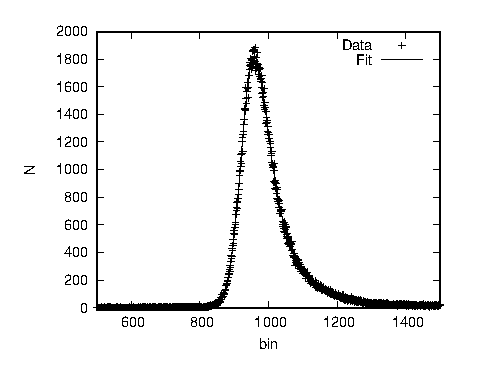
\includegraphics[width=\textwidth]{evaluation_kilian/temp/na_roomtemp.eps}
    \caption{$\SI{27}{\celsius}$}
  \end{subfigure}%
  \begin{subfigure}[h]{0.49\textwidth}
    \centering
    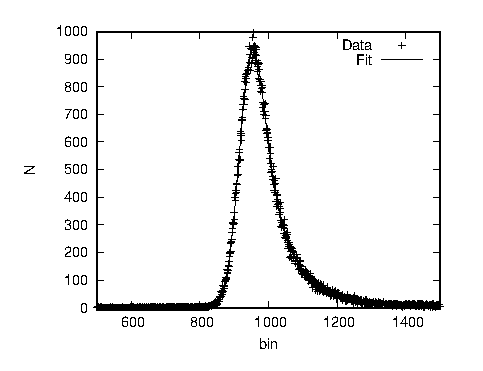
\includegraphics[width=\textwidth]{evaluation_kilian/temp/na_55.eps}
    \caption{$\SI{55}{\celsius}$}
  \end{subfigure}
  \begin{subfigure}[h]{0.49\textwidth}
    \centering
    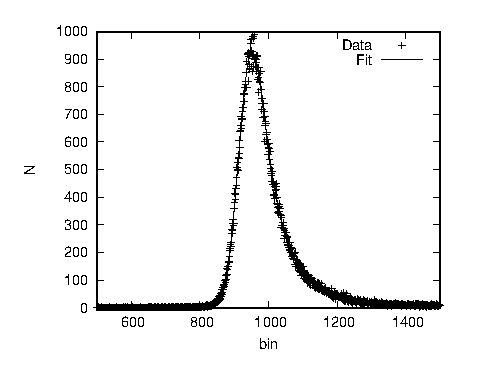
\includegraphics[width=\textwidth]{evaluation_kilian/temp/na_61.eps}
    \caption{$\SI{61}{\celsius}$}
  \end{subfigure}
  \begin{subfigure}[h]{0.49\textwidth}
    \centering
    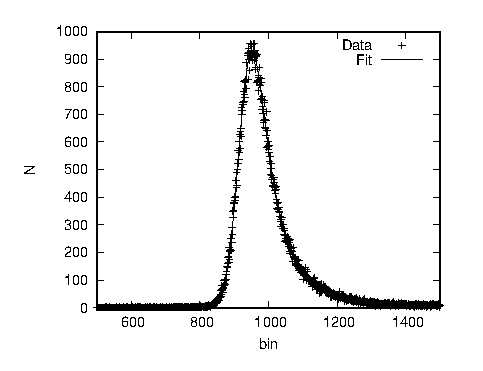
\includegraphics[width=\textwidth]{evaluation_kilian/temp/na_68.eps}
    \caption{$\SI{68}{\celsius}$}
  \end{subfigure}
  \begin{subfigure}[h]{0.49\textwidth}
    \centering
    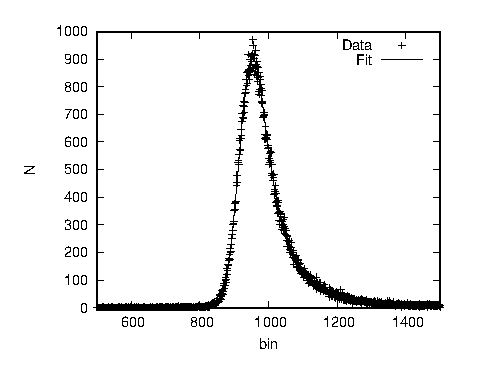
\includegraphics[width=\textwidth]{evaluation_kilian/temp/na_78.eps}
    \caption{$\SI{78}{\celsius}$}
  \end{subfigure}
  \begin{subfigure}[h]{0.49\textwidth}
    \centering
    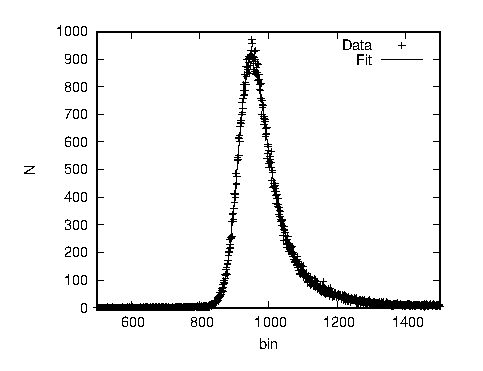
\includegraphics[width=\textwidth]{evaluation_kilian/temp/na_81.eps}
    \caption{$\SI{81}{\celsius}$}
  \end{subfigure}
  \end{figure}
  \begin{figure}\ContinuedFloat
  \begin{subfigure}[h]{0.49\textwidth}
    \centering
    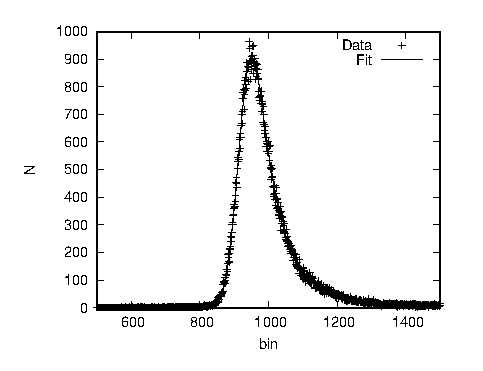
\includegraphics[width=\textwidth]{evaluation_kilian/temp/na_95.eps}
    \caption{$95^\circ$}
  \end{subfigure}
  \begin{subfigure}[h]{0.49\textwidth}
    \centering
    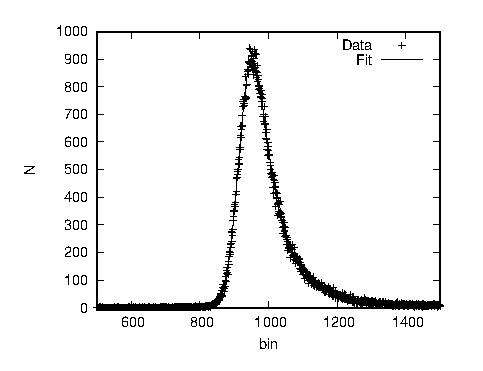
\includegraphics[width=\textwidth]{evaluation_kilian/temp/na_108.eps}
    \caption{$108^\circ$}
  \end{subfigure}
  \begin{subfigure}[h]{0.49\textwidth}
    \centering
    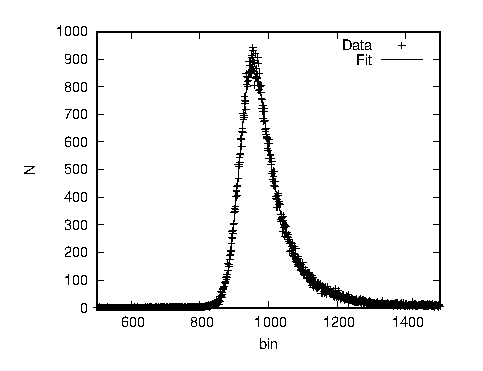
\includegraphics[width=\textwidth]{evaluation_kilian/temp/na_121.eps}
    \caption{$121^\circ$}
  \end{subfigure}
  \caption{Positron lifetime spectra at different temperatures. The error for the temperature is $\SI{1}{\celsius}$.}
  \label{fig:lifetime_spectra}
\end{figure} 

